\begin{figure*}
  %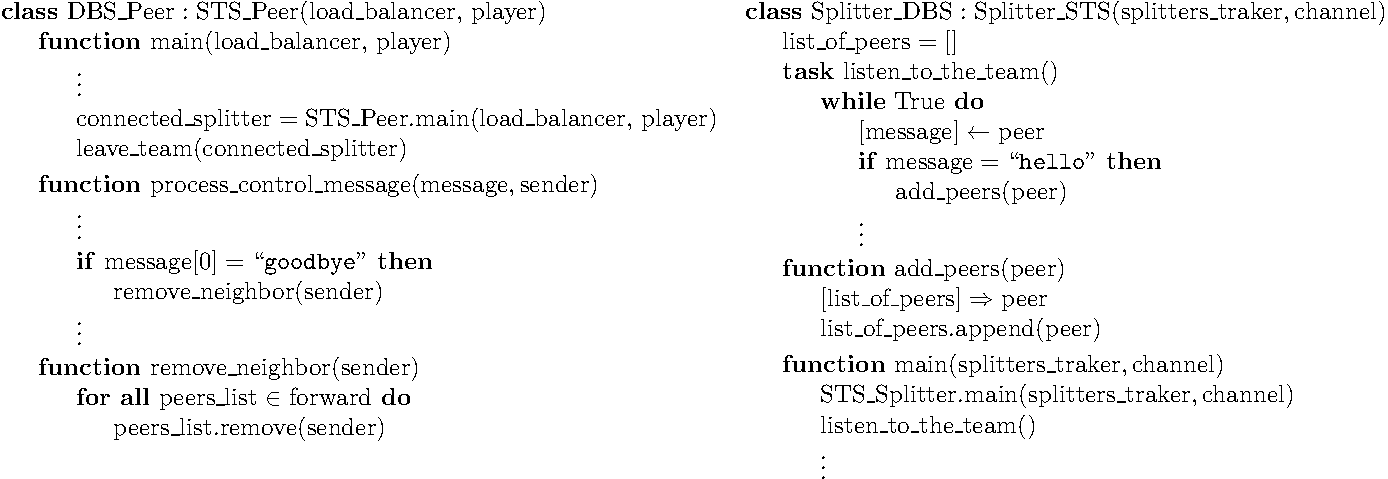
\includegraphics[width=0.55\textwidth]{leaving}
  \fig{300}{4cm}{leaving}
  \caption{Tasks run when an peer $P^t_o$ wants to leave its team
    $T^t$. $P^t_k$ is a neighbor of $P^t_o$ and $S^t$ is the splitter
    of $T^t$.\label{fig:leaving}}
\end{figure*}
An outgoing peer $P^t_o$ (see Fig.~\ref{fig:leaving}) must to: (1) say
$[\mathtt{goodbye}]$ to $S^t$ and to $T^t_o$ (in this order), (2)
relay any pending (received but yet not sent) chunks, and (3) wait for
a $[\mathtt{goodbye}]$ from $S^t$, which performs $T^t = T^t \setminus
P^t_o$. In case of a timeout, $P^t_o$ resets the leaving procedure,
for a maximum number of times.

When a $P^t_k$ receives a $[\mathtt{goodbye}]$ from $P^t_o$, $P^t_k$
removes $P^t_o$ from its neighbors set, by running $T^t_k = T^t_k
\setminus P^t_o$.
